% !TEX root = ../main.tex
\section{Double markup-problemet (dobbel marginalisering)}\label{thr:double-markup-problem}

\paragraph{Definisjon.} \emph{Double markup} (successive monopolies, dobbel marginalisering) oppstår når to suksessive monopolister -- en oppstrøms produsent og en nedstrøms distributør -- begge legger en markup over marginal kostnad. Resultatet er en sluttforbrukerpris som er \emph{høyere} og et kvantum som er \emph{lavere} enn det som maksimerer samlet verdikjedeprofitt. Vertikal integrasjon løser problemet ved å eliminere den ene markupen. [SLIDE]

\subsection*{Forklaring}

BSZ kap.\ 19 presenterer double markup som et uavhengig argument for vertikal integrasjon -- uavhengig av hold-up og free-riding. [SLIDE/BOK]

\textbf{Mekanisme (numerisk eksempel):}
\begin{enumerate}\setlength{\itemsep}{2pt}
\item Oppstrøms produsent $U$ har marginalkostnad $c=20$.
\item Nedstrøms distributør $D$ har kun distribusjonskostnad $=0$ for enkelhet.
\item Sluttetterspørsel: $P = 100 - Q$.
\item $U$ priser overfor $D$ som monopolist: $P_w = 60$ (halvveis mellom $c$ og chokeprisen).
\item $D$ tar $P_w=60$ som sin ``kostnad'' og priser overfor konsumenter som monopolist: $P_{\text{slutt}} = 80$.
\item \textbf{Kvantum $Q=20$, samlet profitt $= (80-20)\cdot 20 = 1{,}200$.}
\end{enumerate}

\textbf{Med vertikal integrasjon:}
\begin{enumerate}\setlength{\itemsep}{2pt}
\item Integrert firma priser direkte: $\max_{Q}\;(100-Q-20)\cdot Q \Rightarrow Q=40$, $P=60$.
\item \textbf{Kvantum $Q=40$, samlet profitt $= (60-20)\cdot 40 = 1{,}600$.}
\end{enumerate}

Integrasjon gir \emph{høyere} profitt (+33\%), \emph{lavere} sluttforbrukerpris (-25\%) og \emph{høyere} kvantum (+100\%). Alle parter (produsent, konsument) er bedre stilt -- \emph{alle vinner}. [BOK]

\textbf{Intuisjon:} Hver monopolist internaliserer ikke effekten av sin markup på den andres etterspørsel. To suksessive markups ``skatter'' etterspørselen to ganger -- en \emph{vertikal eksternalitet}. [SLIDE]

\subsection*{Kjerneforutsetninger}
\begin{itemize}
\item Begge ledd har markedsmakt (monopol eller dominant posisjon).
\item Kvantitet/pris i hvert ledd settes \emph{uavhengig} (Cournot/Stackelberg-struktur).
\item Ingen perfekt kontraktsløsning mellom $U$ og $D$ (ellers kunne man replisere integrasjonsutfallet med kontrakt).
\item Lineære priser (per-enhet wholesale price) -- med twopart tariff ($T + P_w \cdot Q$) kan $U$ ekstrahere surplus uten å vri pris, og double markup forsvinner.
\end{itemize}

\subsection*{Muligheter}
\begin{itemize}
\item Gir et \emph{effektivitetsargument} for vertikal integrasjon som selv konkurransemyndigheter aksepterer (lavere pris til forbruker).
\item Forklarer to-part-tariffer, RPM, franchise fees og andre mellomformer som løser problemet uten full integrasjon.
\item Predikerer at vertikale fusjoner i double-monopoly-industrier kan godkjennes av kartellmyndigheter.
\end{itemize}

\subsection*{Begrensninger og kritikk}
\begin{itemize}
\item Forutsetter markedsmakt i \emph{begge} ledd -- med konkurranse i nedstrøms (mange distributører) forsvinner $D$s markup, og problemet er irrelevant.
\item Two-part tariffer, franchise fees og RPM kan løse double markup kontraktuelt uten integrasjon.
\item Modellen ignorerer stordriftsfordeler, synergier og koordinasjonsgevinster som også motiverer integrasjon.
\item Statisk: ignorerer entry og dynamisk konkurranse.
\end{itemize}

\subsection*{Modell / illustrasjon}

\begin{figure}[H]
\centering
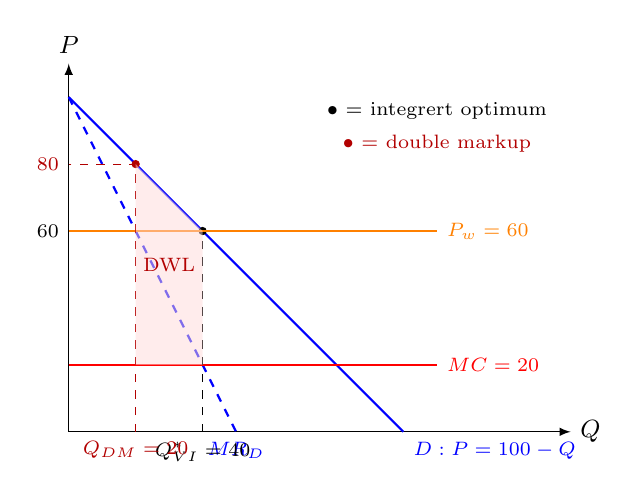
\begin{tikzpicture}[>=latex, scale=0.85, every node/.style={font=\small}]
  % Akser
  \draw[->] (0,0) -- (7.5,0) node[right] {$Q$};
  \draw[->] (0,0) -- (0,5.5) node[above] {$P$};
  % Etterspørsel P=100-Q skalert: P/20 og Q/10
  \draw[thick, blue] (0,5) -- (5,0) node[below right] {\scriptsize $D: P=100-Q$};
  % MR for etterspørsel
  \draw[thick, blue, dashed] (0,5) -- (2.5,0) node[below] {\scriptsize $MR_D$};
  % MC = 20 => 1.0 i skala
  \draw[thick, red] (0,1.0) -- (5.5,1.0) node[right] {\scriptsize $MC=20$};
  % Integrert optimum: Q=40, P=60
  \filldraw[black] (2.0,3.0) circle (1.5pt);
  \draw[dashed] (2.0,0) -- (2.0,3.0) -- (0,3.0);
  \node[below] at (2.0,0) {\scriptsize $Q^{*}_{VI}=40$};
  \node[left] at (0,3.0) {\scriptsize $60$};
  % Double markup: Pw=60, P_slutt=80, Q=20
  \draw[thick, orange] (0,3.0) -- (5.5,3.0) node[right] {\scriptsize $P_w=60$};
  % MR for D facing Pw=60: D's MR = 100-2Q, men D ser P_w som MC
  % D's optimum: MR_D = P_w => 100-2Q=60 => Q=20
  \filldraw[red!70!black] (1.0,4.0) circle (1.5pt);
  \draw[dashed, red!70!black] (1.0,0) -- (1.0,4.0) -- (0,4.0);
  \node[below, red!70!black] at (1.0,0) {\scriptsize $Q_{DM}=20$};
  \node[left, red!70!black] at (0,4.0) {\scriptsize $80$};
  % Shading dødvektstap
  \fill[red!15, opacity=0.5] (1.0,4.0) -- (2.0,3.0) -- (2.0,1.0) -- (1.0,1.0) -- cycle;
  \node[font=\scriptsize, red!70!black] at (1.5,2.5) {DWL};
  % Legend
  \node[font=\scriptsize] at (5.5,4.8) {$\bullet$ = integrert optimum};
  \node[font=\scriptsize, red!70!black] at (5.5,4.3) {$\bullet$ = double markup};
\end{tikzpicture}
\caption{\textbf{Double markup.} Med to uavhengige monopolister (oppstrøms og nedstrøms) ender sluttprisen på 80 med kvantum 20 (rødt punkt). Vertikal integrasjon gir $P=60$, $Q=40$ (svart punkt) -- lavere pris, høyere kvantum, eliminert dødvektstap (DWL). [BOK -- BSZ kap.\ 19]}
\end{figure}

\subsection*{Numerisk oppsummering}

\begin{center}
\renewcommand{\arraystretch}{1.15}
\begin{tabular}{@{}lccc@{}}
\toprule
 & \textbf{Double markup} & \textbf{Integrert} & \textbf{Endring} \\
\midrule
$P_{\text{slutt}}$ & 80 & 60 & $-25\%$ \\
$Q$ & 20 & 40 & $+100\%$ \\
Samlet profitt & 1{,}200 & 1{,}600 & $+33\%$ \\
Konsumentoverskudd & 200 & 800 & $+300\%$ \\
\bottomrule
\end{tabular}
\end{center}

\subsection*{Eksempler}
\begin{itemize}\setlength{\itemsep}{2pt}
\item \textbf{Farmasøytisk industri.} Legemiddelprodusent med patentmonopol selger til apotekkjeder med lokal markedsmakt. Begge legger markup -- pasienter betaler mer enn nødvendig. Løsning i Skandinavia: regulerte apotekpriser (RPM-variant) eller parallelimport. [EKS]
\item \textbf{Internettleverandører og innholdsleverandører.} ISP (monopolist i siste mil) og Netflix (dominant innhold) priset uavhengig -- double markup drev opp priser for forbrukere. Løst delvis via peering-avtaler og bundling. [EKS]
\end{itemize}

\subsection*{Kobling til søyle og andre teorier}
Søyle: \SOne\ (eierskap fjerner vertikal eksternalitet), \SThree\ (kontraktsdesign som alternativ til integrasjon). Relaterte: \thref{vertical-integration-outsourcing}{Vertikal integrasjon og outsourcing}, \thref{vertical-integration-market-power}{VI og market power}, \thref{externalities}{Eksternaliteter}, \thref{transfer-pricing}{Transfer pricing} (internpris kan settes til MC og eliminere dobbel markup).

\paragraph{Brukt i spørsmål:} Q12 (primært), Q11 (referert).
